\chapter{Linear elasticity solver}
\label{s:elasticity}

\section{Synopsis}
The LinearElasticSolver is a solver for solving the linear elasticity equations
in two and three dimensions. Whilst this may be suitable for simple solid
mechanics problems, its main purpose is for use for mesh deformation and
high-order mesh generation, whereby the finite element mesh is treated as a
solid body, and the deformation is applied at the boundary in order to curve the
interior of the mesh.

Currently the following equation systems are supported:
%
\begin{center}
\begin{tabular}{lp{8cm}}
  \toprule
  Value & Description \\
  \midrule
  \inltt{LinearElasticSystem} & Solves the linear elastic equations. \\
  \inltt{IterativeElasticSystem} & A multi-step variant of the elasticity solver,
                                   which breaks a given deformation into multiple
                                   steps, and applies the deformation to a mesh. \\
  \bottomrule
\end{tabular}
\end{center}

\subsection{The linear elasticity equations}

The linear elasticity equations model how a solid body deforms under the
application of a `small' deformation or strain. The formulation starts with the
equilibrium of forces represented by the equation
%
\begin{equation}
\nabla \cdot \mathbf{S} + \mathbf{f} = \mathbf{0} \quad \textrm{in} \quad \Omega
\label{eq:strong}
\end{equation}
%
where $\mathbf{S}$ is the stress tensor and $\mathbf{f}$ denotes a
spatially-varying force. We further assume that the stress tensor $\mathbf{S}$
incorporates elastic and, optionally, thermal stresses that can be switched on
to assist in mesh deformation applications. We assume these can be decomposed so
that $\mathbf{S}$ is written as
%
\[
\mathbf{S} = \mathbf{S}_e + \mathbf{S}_t,
\]
%
where the subscripts $e$ and $t$ denote the elastic and thermal terms
respectively. We adopt the usual linear form of the elastic stress tensor as
%
\[
\mathbf{S}_e = \lambda\mbox{Tr}(\mathbf{E}) \, \mathbf{I} +\mu \mathbf{E},
\]
%
where $\lambda$ and $\mu$ are the Lam\'e constants, $\mathbf{E}$ represents the
strain tensor, and $\mathbf{I}$ is the identity tensor. For small deformations,
the strain tensor $\mathbf{E}$ is given as
%
\begin{equation}
\mathbf{E} =\frac{1}{2} \left ( \nabla \mathbf{u}+ \nabla \mathbf{u}^t \right )
\end{equation}
%
where $\mathbf{u}$ is the two- or three-dimensional vector of displacements. The
boundary conditions required to close the problem consist of prescribed
displacements at the boundary $\partial \Omega$, i.e.
\begin{equation}
  \mathbf{u} = \hat{\mathbf{u}} \quad \textrm{in}\ \partial \Omega.
\end{equation}

We further express the Lam\'e constants in terms of the Young's modulus $E$ and
Poisson ratio $\nu$ as
%
\[
\lambda = \frac{\nu E}{(1+\nu)(1-2\nu)}, \qquad \mu = \frac{E}{2(1+\nu)}.
\]
%
The Poisson ratio, valid in the range $\nu < \tfrac{1}{2}$, is a measure of the
compressibility of the body, and the Young's modulus $E > 0$ is a measure of its
stiffness.

\section{Usage}
\begin{lstlisting}[style=BashInputStyle]
LinearElasticSolver [arguments] session.xml [another.xml] ...
\end{lstlisting}

\section{Session file configuration}
\subsection{Solver Info}
\begin{itemize}
  \item \inltt{EqType} Specifies the PDE system to solve, based on the choices
  in the table above.
  \item \inltt{Temperature} Specifies the form of the thermal stresses to
  use. The choices are:
  \begin{itemize}
    \item \inltt{None}: No stresses (default).
    \item \inltt{Jacobian}: Sets $\mathbf{S}_t = \beta JI$, where $\beta$ is a
    parameter defined in the parameters section, $J$ is the elemental Jacobian
    determinant and $I$ is the identity matrix.
    \item \inltt{Metric}: A more complex term, based on the eigenvalues of the
    metric tensor. This can only be used for simplex elements (triangles and
    tetrahedra). Controlled again by the parameter $\beta$.
  \end{itemize}
  \item \inltt{BCType} Specifies the type of boundary condition to apply when
  the \inltt{IterativeElasticSystem} is being used.
  \begin{itemize}
    \item \inltt{Normal}: The boundary conditions are split into
    \inltt{NumSteps} steps, as defined by a parameter in the session file
    (default).
    \item \inltt{Repeat}: As the geometry is updated, re-evaluate the boundary
    conditions. This enables, for example, a cirlce to be rotated continuously.
  \end{itemize}
\end{itemize}

\subsection{Parameters}

The following parameters can be specified in the \inltt{PARAMETERS} section of
the session file:
\begin{itemize}
  \item \inltt{nu}: sets the Poisson ratio $\nu$.\\ 
  \textit{Default value}: 0.25.
  \item \inltt{E}: sets the Young's modulus $E$.\\ 
  \textit{Default value}: 1.
  \item \inltt{beta}: sets the thermal stress coefficient $\beta$.\\ 
  \textit{Default value}: 1.
  \item \inltt{NumSteps}: sets the number of steps to use in the case that the
  iterative elastic system is enabled. Should be greater than 0.\\ 
  \textit{Default value}: 0.
\end{itemize}

\section{Examples}

\subsection{L-shaped domain}

The first example is the classic L-shaped domain, in which an exact solution is
known, which makes it an ideal test case~\cite{Ko07}. The domain is the polygon
formed from the vertices
%
\[
(-1,-1), (0,-2), (2,0), (0,2), (-1,-1), (0,0).
\]
%
The exact solution for the displacements is known in polar co-ordinates
$(r,\theta)$ as
%
\begin{align*}
  u_r(r,\theta) &= \frac{r^\alpha}{2\mu} \left[
    C_1(C_2 - \alpha - 1)\cos((\alpha-1)\theta) - (\alpha+1)\cos((\alpha+1)\theta)
  \right]\\
  u_\theta(r,\theta) &= \frac{r^\alpha}{2\mu} \left[
    (\alpha+1)\sin((\alpha+1)\theta) + C_1(C_2+\alpha-1)\sin((\alpha-1)\theta)
  \right]
\end{align*}
%
where $\alpha\approx 0.544483737\dots$ is the solution of the equation
$\alpha\sin(2\omega) + \sin(2\omega\alpha) = 0$, 
%
\[
C_1 = -\frac{\cos((\alpha+1)\omega)}{\cos((\alpha-1)\omega)},\qquad
C_2 = 2\frac{\lambda + 2\mu}{\lambda+\mu}
\]
with $\lambda$ and $\mu$ being the Lam\'e constants and $\omega = 3\pi/4$.
Boundary conditions are set to be the exact solution and
$\mathbf{f} = \mathbf{0}$. The solution has a singularity at the origin, and so
in order to test convergence $h$-refinement is required.

\begin{figure}
  \begin{center}
    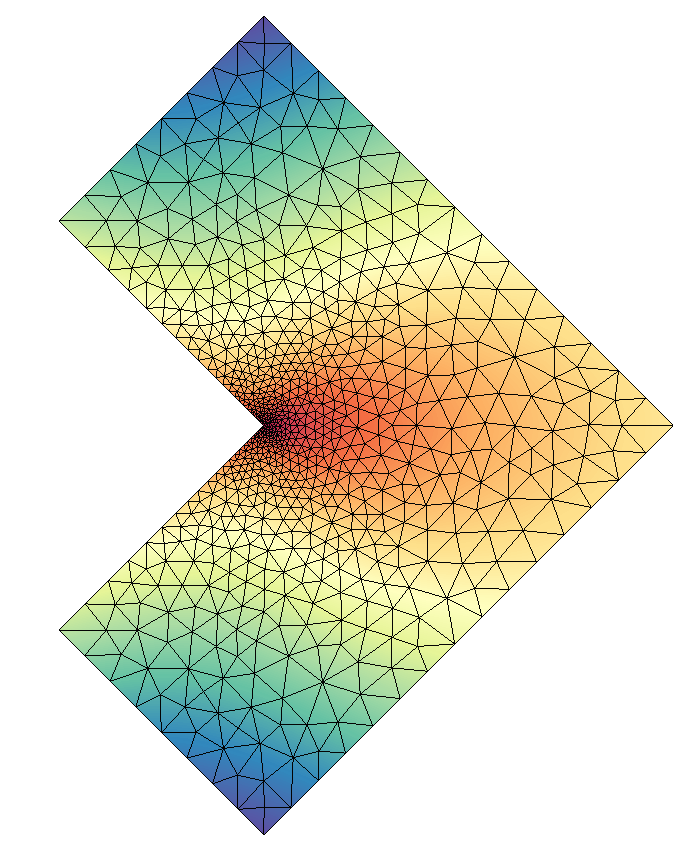
\includegraphics[width=0.5\textwidth]{Figures/l-shape}
  \end{center}
  \caption{Solution of the $u$ displacement field for the L-shaped domain.}
  \label{fig:elas:ldomain}
\end{figure}

A simple example of how the linear elastic solver can be set up can be found in
the \inlsh{Tests/L-shaped.xml} session file in the linear elastic solver
directory. A more refined domain with the obtained $u$ solution is shown in
figure~\ref{fig:elas:ldomain}. The solver can be run using the command:

\begin{lstlisting}[style=BashInputStyle]
  LinearElasticSolver L-domain.xml
\end{lstlisting}

The obtained solution \inlsh{L-domain.fld} can be applied to the mesh to obtain
a deformed XML file using the \inltt{deform} module in \inltt{FieldConvert}:

\begin{lstlisting}[style=BashInputStyle]
  FieldConvert -m deform L-domain.xml L-domain.fld L-domain-deformed.xml
\end{lstlisting}

\subsection{Boundary layer deformation}

In this example we use the iterative elastic system to apply a large deformation
to a triangular boundary layer mesh of a square mesh $\Omega = [0,1]^2$. At the
bottom edge, we apply a Dirichlet condition $g=\tfrac{1}{2}\sin(\pi x)$ that is
enforced by splitting it into $N$ substeps, so that at each step we solve the
system with the boundary condition $g^n(x) = g(x)/N$. The process is depicted in
figure~\ref{fig:elas:bl}.

\begin{figure}
  \begin{center}
    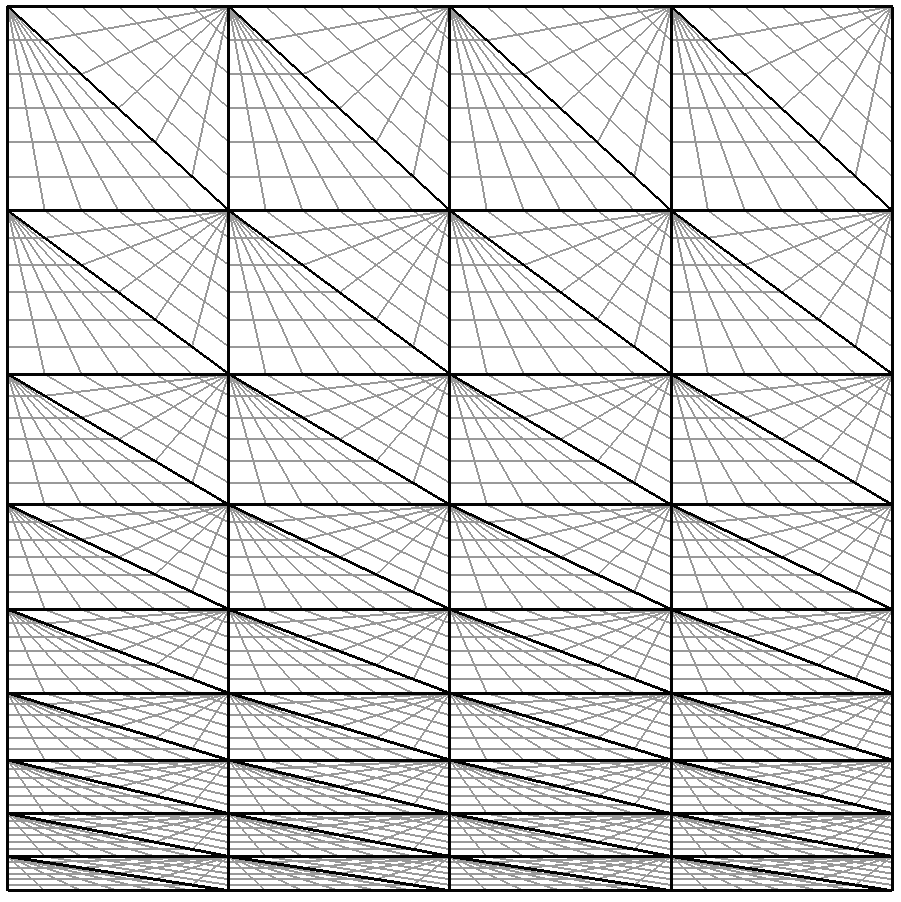
\includegraphics[width=0.3\textwidth]{Figures/bl-0}
    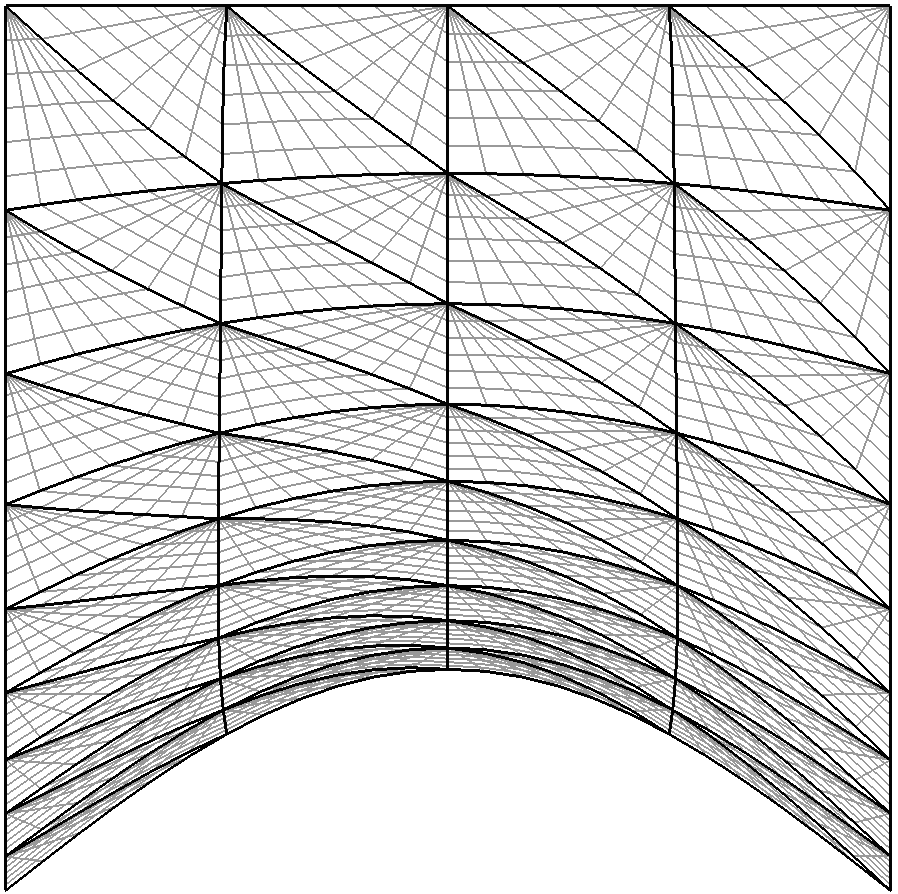
\includegraphics[width=0.3\textwidth]{Figures/bl-1}
    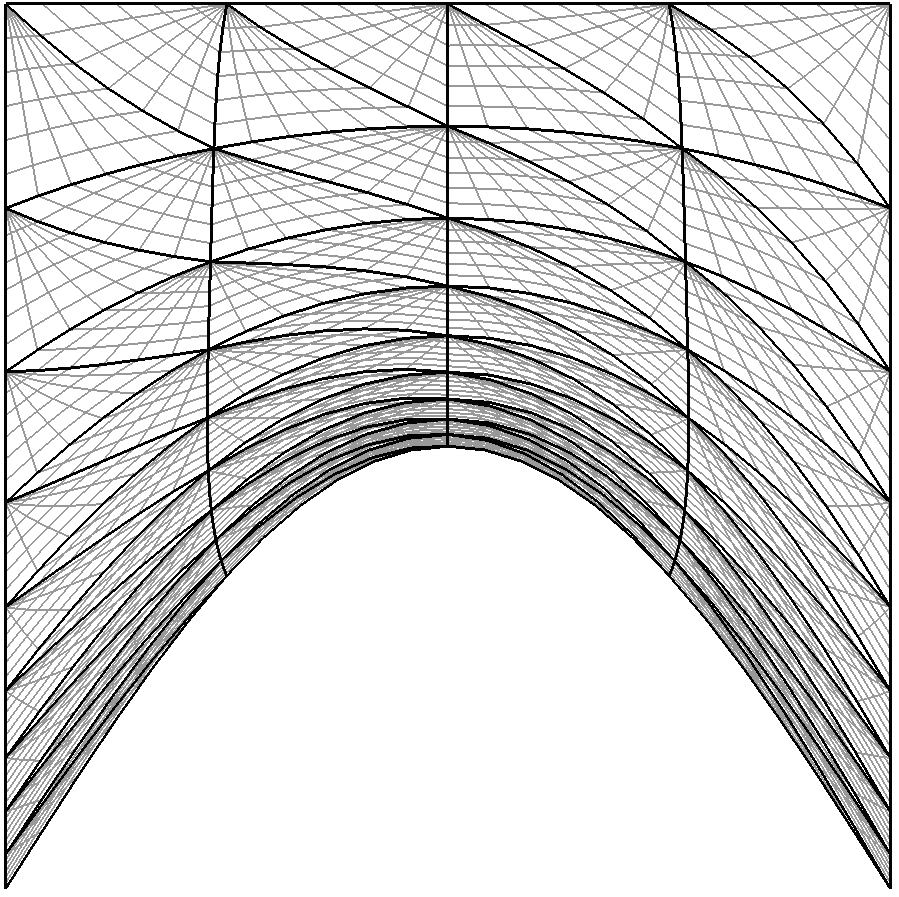
\includegraphics[width=0.3\textwidth]{Figures/bl-2}
  \end{center}
  \caption{Figures that show the initial domain (left), after 50 steps (middle)
    and final deformation of the domain (right).}
  \label{fig:elas:bl}
\end{figure}

The setup is very straightforward. The geometry can be found inside the file
\inlsh{Examples/bl-mesh.xml} and the conditions inside
\inlsh{Examples/bl-conditions.xml}. The solver can be set up using the following
parameters, with \inltt{NumSteps} denoting $N$:

\begin{lstlisting}[style=XMLStyle]
  <SOLVERINFO>
    <I PROPERTY="EQTYPE" VALUE="IterativeElasticSystem" />
  </SOLVERINFO>
  
  <PARAMETERS>
    <P> nu       = 0.3 </P>
    <P> E        = 1.0 </P>
    <P> NumSteps = 100 </P>
  </PARAMETERS>
\end{lstlisting}

To identify the boundary that we intend to split up into substeps, we must
assign the \inltt{WALL} tag to our boundary regions:

\begin{lstlisting}[style=XMLStyle]
  <BOUNDARYCONDITIONS>
    <REGION REF="0">
      <D VAR="u" VALUE="0" USERDEFINEDTYPE="Wall" />
      <D VAR="v" VALUE="0.5*sin(PI*x)" USERDEFINEDTYPE="Wall" />
    </REGION>
    <REGION REF="1">
      <D VAR="u" VALUE="0" />
      <D VAR="v" VALUE="0" />
    </REGION>
  </BOUNDARYCONDITIONS>
\end{lstlisting}

The solver can then be run using the command:

\begin{lstlisting}[style=BashInputStyle]
  LinearElasticSolver bl-mesh.xml bl-conditions.xml
\end{lstlisting}

This will produce a series of meshes \inlsh{bl-mesh-\%d.xml}, where \%d is an
integer running between 0 and 100. If at any point the mesh becomes invalid,
that is, a negative Jacobian is detected, execution will cease.

%%% Local Variables:
%%% mode: latex
%%% TeX-master: "../user-guide"
%%% End:
